\documentclass[12pt]{article}

%%%%%%%%%%%%%%%%%%%%%%% Don't change anything in here. This space is called the preamble, it is where you tell the computer to load the proper LaTeX packages to perform the math and formatting desired. 
\usepackage[tmargin=1in,bmargin=1in,lmargin=1.25in,rmargin=1.25in]{geometry}
\usepackage{physics} 
\usepackage{siunitx} 
\usepackage{enumerate} 
\usepackage{pgfplots}
\usepackage{pgfplotstable}
\usepackage{tikz,pgfplots}
\usepackage{amsmath}  %I added this so that you can use the align tool for equations!
\usepackage{wasysym} %This package allows you to put emojis in your paper!!!!
	%wasysym: \smiley{} \frownie{} see http://milde.users.sourceforge.net/LUCR/Math/mathpackages/wasysym-symbols.pdf for list of most symbols available in this package
\usepackage{graphicx}
\usepackage{array}
\usepackage{amssymb}
\usepackage{geometry}
 \geometry{
 a4paper,
 total={170mm,257mm},
 left=20mm,
 top=10mm,
 }



\pgfplotsset{compat=1.14}
%%%%%%%%%%%%%%%%%%%%%%%%% Again, Don't change anything Above %%%%%%%%%%%%%%%%%%%%

\begin{document}

\title{An analysis on the definitions of “AI System”} %Title should be concise and to the point 
\author{Executive summary - Alessandro Lorenzi, Luca Cazzola} %Your name first


% \date{\today}  % This will automatically put today's date in the report
\date{}

\maketitle  %this command makes the title

%%%% to use this template, please copy-paste the entire thing into a new document and save it so you have it!

%%%%% If you want to omit something in this lab, place a % sign to the left of it and it won't show up on the lab, like this line!

% \begin{abstract} 
% 	The abstract should be a short 3-5 sentence paragraph. In it, you should state the hypothesis, what you did, and what you found. The abstract is meant to be a very short summary of your paper to follow. It is a good suggestion to write the abstract last in your report after you have written everything else. This will allow you to best summarize your work. 
% \end{abstract}
% \vspace{-1 in} % adjust the length to suit your aesthetic 
\section{The problem}
	 
In the contemporary context, delineating precisely what constitutes an Artificial Intelligence system (AI system) has assumed utmost importance. As technology swiftly advances and permeates various facets of our daily routines, the distinctions between conventional computing and artificial intelligence continue to blur. Establishing a clear and comprehensive definition for AI systems is crucial for several reasons. First and most important, to create effective regulations not just for the design and for the correct use of AI systems, but also for the entering into the market of these technologies. That leads to legal interpretation and enforcement. Furthermore, specifying which techniques are under the scope of AI, ensures the public has a clear understanding of what AI is, avoiding or mitigation issues related to both the underused and overused of AI systems. Last but not least, a well-defined concept of AI is essential for establishing ethical guidelines.


    
    %note the cite above. That is an in text citation. By putting citations in your bibliography, you can cite in text simply using the \cite{} command and putting the number of the citation in the {} 
    

    
\section{The analysis}
% \begin{table}[h]
% \begin{tabular}{|>{\tiny\bfseries\raggedright\arraybackslash}m{2.5cm}|*{6}{>{\centering\arraybackslash}m{1.9cm}|}}
% \hline
% \tiny\textbf{} & \tiny\textbf{AI EU GROUP} & \tiny\textbf{COMMISSION} & \tiny\textbf{COUNCIL} & \tiny\textbf{PARLIAMENT} & \tiny\textbf{OECD} & \tiny\textbf{FLORIDI $^{(1)}$} \\
% \hline
% SOFTWARE & \checkmark$^{(2)}$ & \checkmark & \checkmark & \checkmark & \checkmark & \checkmark \\
% \hline
% HARDWARE & & & \checkmark & \checkmark & \checkmark & \checkmark \\
% \hline
% AUTONOMY & & & \checkmark & \textit{“varying levels”} & \textit{“varying levels”} & \checkmark \\
% \hline
% HUMAN DEFINED OBJECTIVES & & \checkmark & \checkmark & & & \\
% \hline
% PREDICTIONS, DECISIONS, RECOMMENDATIONS IN OUTPUT & & \checkmark & \checkmark & \checkmark & \checkmark & \checkmark \\
% \hline
% CONTENT IN OUTPUT & & \checkmark & \checkmark & & \checkmark & \checkmark \\
% \hline
% REFERENCES TO AI TECHNIQUES & & \textit{Annex 1} & \checkmark$^{(3)}$ & & & \\
% \hline
% PROCESS INFORMATION & \checkmark & & \checkmark & & \checkmark & \checkmark \\
% \hline
% INFLUENCE AND INTERACT WITH ENVIRONMENT & \checkmark & \checkmark & \checkmark & \checkmark & \checkmark & \checkmark \\
% \hline
% \end{tabular}
% \end{table}
% \begin{itemize}
%     \tiny\item (1): Floridi, Luciano, On the Brussels-Washington consensus about the legal definition of Artificial Intelligence (December 3, 2023)
%     \item (2): Only human designed
%     \item (3): Programming approaches that execute operations automatically
% \end{itemize}
% \newline
In order to determine, from both a legal and technological standpoint, which definition would be the most appropriate, we have conducted an analysis of the structure, differences, and common points of the formulations provided by various organizations. Particular focus has been given to the European High-Level Expert Group on AI (2018 version), the European Commission, Council and Parliament working on the AI Act draft, the OECD Artificial Intelligence Policy Observatory (OECD.AI) and to the Luciano Floridi proposal in the “On the Brussels-Washington consensus about the legal definition of Artificial Intelligence” paper (2023).
In the next page the first image reported the summarize table of the analysis, the bold column contains the most common and important concepts included into the different formulations of “AI System”. The check mark indicates the presence of the concept in the definition by the corresponding organization.
The second table instead shows a list of real cases applied to the previous definitions, to understand if there are systems mistakenly recognized as AI systems, or vice versa, if they are ignored even though they are AI. Note here that if the color is green, both the "x" and check marks are positive. 


\begin{figure}[ht]
  \centering
  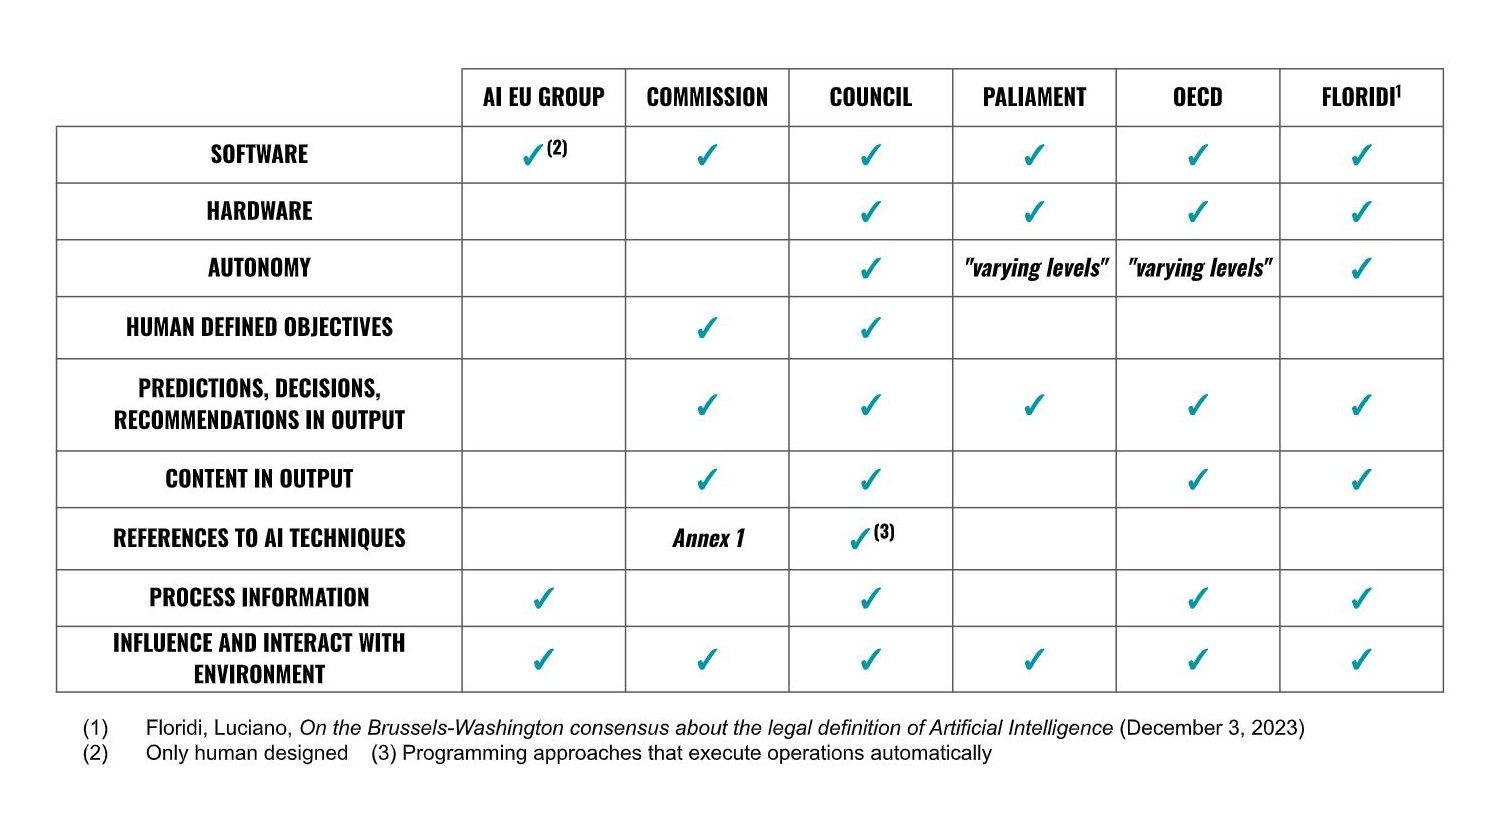
\includegraphics[width=135mm]{img/aa-1.jpg}
  \caption{Analysis on different definitions.}
  \vspace{1em} % Adjust the vertical space between the images
  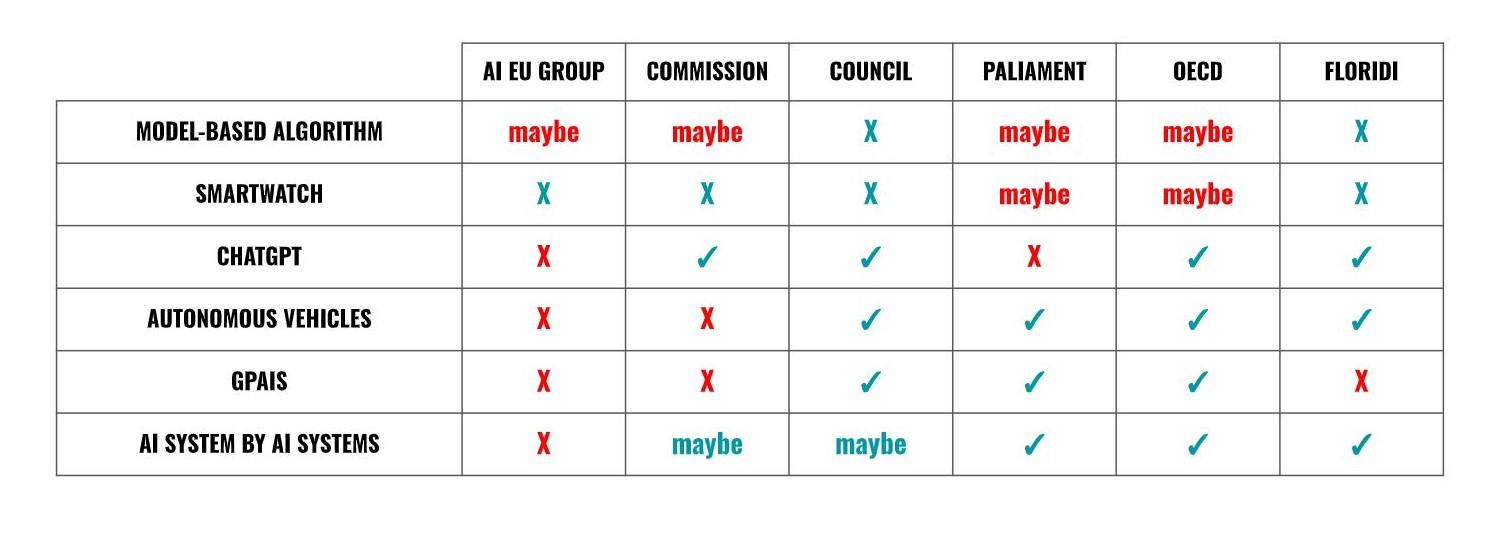
\includegraphics[width=135mm]{img/aa-3.jpg}
  \caption{Real case application of the definitions.}
\end{figure}

\section{Conclusion}
This report shows that most of the explanations presented contain issue or ambiguity in at least one of the points considered. However, the best definition seems to be the Floridi's one: \textit{“Artificial Intelligence (AI) refers to an engineered system that can, for a given set of human-defined objectives, generate outputs – such as content, predictions, recommendations, or decisions – learn from historical data, improve its own behaviour, and influence people and environments”}. In the last column of both the tables, in fact, there is a higher number of green check marks. That is the sole option that encompasses all the most pertinent attributes of AI Systems, specifically the transformative and autonomous variants, without being excessively broad or specific. Furthermore, highlighting the ability to learn from experience and improve behavior, there is a distinct distinction between simple model-based algorithms (not AI) and systems that we consider artificial intelligence.
Even though some concepts, such as the “human-defined objectives”, aren't really clear and other issues can pop up, we can still conclude that, from a technical standpoint, this definition seems to be the most appropriate for defining what an AI system is.      
    
%%%%%%%%%%%%%%%%%%%%%%%%%%%%%%%%%%%%%%%%%%%%%%%%%%%%%%%%%%%%%%%%%%%%%%%%%%%%%%%%%%%%%
%%%% This is the Bibliography where you will cite your sources used in the paper %%%%

% \begin{thebibliography}{0}

% 	%Each item starts with a \bibitem{} command and the details thereafter.
	
% 	\bibitem{1} Cite your first source here
% 	\bibitem{2} Cite another source
	
%     %%% The 1,2 etc. are used to cite in text. See up in the intro for an example
%     %%% When you want to cite in your cite, type in \cite{} wherever you want
% \end{thebibliography}
    
%%%%%%%%%%%%%%%%%%%%%%%%%%%%%%%%%%%%%%%%%%%%%%%%%%%%%%%%%%%%%%%%%%%%%%%%%%%%%%%%%%%%    


%%%%%%%%%%%%%%%%%%%%%%%%%%%%%%%%%%%%%%%%%%%%%%%%%%%%%%%%%%%%%%%%%%%%%%%%%%%%%%%%%%%%%

% Here are some equations and other useful things, feel free to copy and paste into your lab report :) %

% Note: It is super easy to look up equations/constants already formatted in LaTeX online. Here are a few websites I like to use:

% LaTeX Tutorial: http://pages.physics.cornell.edu/sps/pages/resources/latex.html
	%NOTE: This contains both pdf and text (code) of each document, which includes guides, lab 			report templates, and lots of other good stuff!

% LaTeX Cheat Sheet: http://wch.github.io/latexsheet/

% Equations: http://www.equationsheet.com/sheets/Equations-5.html

% Constants, symbols, letters, etc:  http://www.rpi.edu/dept/arc/training/latex/LaTeX_symbols.pdf

% AP Physics Calculus Reference Table: https://secure-media.collegeboard.org/digitalServices/pdf/ap/physics-c-tables-and-equations-list.pdf

% AP Physics Trig Reference Table: https://secure-media.collegeboard.org/digitalServices/pdf/ap/ap-physics-1-equations-table.pdf

% Regents Physics Reference Table: http://www.p12.nysed.gov/assessment/reftable/physics-rt/physics06tbl.pdf

% Here are three good sources to use other then this for considering how to write a good lab report. Much of this guide was gleaned from them
	
    %http://web.mit.edu/8.13/www/Samplepaper/simple-zipped/simple-paper.pdf 				-MIT Physics Lab (really, really good template!) 
    
    % http://pages.physics.cornell.edu/sps/pages/resources/LatexSession/Exercises/LabReport.pdf -Cornell Template
    % https://engineering.purdue.edu/ME588/LabManual/report_format.pdf 							-Purdue Engineering Template 
    % http://physics.columbia.edu/files/physics/content/1291_report_format_and_example.pdf 		-Columbia University Template
    % https://www.baylor.edu/physics/doc.php/110769.pdf											-Baylor University Template
    % www.nd.edu/~hgberry/Fall2012/Guidelines.docx												-Notre Dame Template
    %http://www.esf.edu/iq/colloquium/documents/LabReportnotes.pdf								-SUNY ESF Template
    %http://writing.engr.psu.edu/workbooks/laboratory.html										-Virginia Tech Template
    %https://projects.ncsu.edu/labwrite/index_labwrite.htm										-SUPER in-depth guide to writing lab reports
    
    %https://gist.github.com/dcernst/1827406													-Template for completing Math homework in LaTeX
    %https://joshldavis.com/2014/02/12/doing-your-homework-in-latex/							-More about math homework in LaTeX
    
    
    
%Purdue University Online Writing Lab-OWL: https://owl.english.purdue.edu/ Use this to generate citations!

%Basically, if you get stuck, just google "Latex ______" for whatever you need and look through the LaTeX stackexchange or wiki article to find and copy/paste what you need





%	Here are some common equations we use in class. I will continue to update as we continue throughout the year. I will attempt to organize by the order we learn the topics from oldest at the top to newest at the bottom. Go ahead and copy/paste as needed in your report

%%%%%%%%%%%%%%%%%%%%%%%%%% Basic Calculus %%%%%%%%%%%%%%%%%%%%%%%%%%%%%%%%%%%%%

%		   $$\frac{\mathrm{d}}{\mathrm{d}x}C=0$$
%           $$\frac{\mathrm{d}}{\mathrm{d}x}Cx=C$$
%           $$\frac{\mathrm{d}}{\mathrm{d}x}x=1$$           
%           $$\frac{\mathrm{d}}{\mathrm{d}x}x^n = nx^{n-1} $$  	-power rule
% 		   $$\frac{\mathrm{d}}{\mathrm{d}x}fg= fg'+f'g$$		-product rule
%           $$\frac{\mathrm{d}}{\mathrm{d}x}f(g(x))=f'(g(x))g'(x)$$	-chain rule
%           $$\frac{\mathrm{d}}{\mathrm{d}x} \sin{x} = \cos{x}$$	
%           $$\frac{\mathrm{d}}{\mathrm{d}x} \cos{x} = -\sin{x}$$
           
%           $$\int k \mathrm{d}x = kx+C$$		-integral of a constant
%           $$\int x^n \mathrm{d}x= \frac{1}{n+1}x^{n+1}+C$$	-power rule for integrals
%           $$\int \cos{u}\mathrm{d}u = \sin{u} + C$$	
%           $$\int \sin{u}\mathrm{d}u = -cos{u} + C$$	

% see https://reu.dimacs.rutgers.edu/Symbols.pdf for a nice list of math LaTeX symbols

%%%%%%%%%%%%%%%%%%%%%%%%%%%%  Kinematics %%%%%%%%%%%%%%%%%%%%%%%%%%%%%%%%%%%%%%%

%			$$\bar{v}=\frac{d}{t}$$ 								-average speed
%			$$v=\frac{\mathrm{d}x}{\mathrm{d}t}$$					-instantaneous velocity definition
%			$$a=\frac{\mathrm{d}v}{\mathrm{d}t}$$					-instantaneous acceleration definition
%			if acceleration is constant, then:
%				$${x_f}={x_i}+{v_i}t+\frac{1}{2}a{t^2}$$  			-free-fall equation
%				$${v_f}={v_i}+at$$									-find new velocity
%				$${{v_f}^2}={{v_i}^2}+2a({x_f}-{x_i})$$				-equation without time

%%%%%%%%%%%%%%%%%%%%%%%%%%%%% Newton's Laws %%%%%%%%%%%%%%%%%%%%%%%%%%%%%%%%%%%%%%

%			$$F_{net}=ma=m\frac{\mathrm{d}v}{\mathrm{d}t}=m\frac{\mathrm{d}^{2}x}{\mathrm{d}{t^2}}$$	-Newt's 2nd Law
%			$$F_f=\mu F_n$$											-Friction 
%			$$w=mg$$												-Weight

%%%%%%%%%%%%%%%%%%%%%%%%%%%%%%%% Work, Power, Energy %%%%%%%%%%%%%%%%%%%%%%%%%%%%%%%%%%%

%			$$W=\Delta E = \int F dx = Fd  \hspace{3pt} \text{(if F constant)} $$ 	-Work-Energy Theorem
%			$$Power=\frac{\mathrm{d}E}{\mathrm{d}t}=\frac{\mathrm{d}W}{\mathrm{d}t} = \frac{Fd}{t} = F \bar{v}$$		-Power
%			$$K=\frac{1}{2}mv^2$$													-Kinetic Energy
%			$$U_g=mgh$$																-Gravitational Potential Energy
%			$$U_e=\frac{1}{2}kx^2$$													-Spring Potential Energy
%			$$F_e=kx$$																-Hooke's Law
%			$$F=-\frac{\mathrm{d}U}{\mathrm{d}x}$$									-Force is derivative of Potential

%%%%%%%%%%%%%%%%%%%%%%%%%%%%%%%%%%%%% Momentum, Center of Mass %%%%%%%%%%%%%%%%%%%%%%%%%%%%%%%%%%%

% 			$$p=mv$$								-definition of momentum
%			$$F=\frac{\mathrm{d}p}{\mathrm{d}t}
%			$$ft=\Delta{p}$$ 						-trig version of impulse momentum theorem
%			$$J=\int F \mathrm{d}t = \Delta{p}$$	-calc version of impulse momentum theorem
%			$$p_{before}=p_{after}$$				-Conservation of Momentum
%			$$X_{c.o.m}=\frac{\Sigma x_i m_i}{M}$$  -x-coordinate of Center of Mass
%       	$$Y_{c.o.m}=\frac{\Sigma y_i m_i}{M}$$  -y-coordinate of Center of Mass


%%%%%%%%%%%%%%%%%%%%%%%%%%%%%%%%%%% Rotational Kinematics %%%%%%%%%%%%%%%%%%%%%%%%%%%%%%%%%%%%%%%

%		$$\omega=\frac{\mathrm{d}\theta}{\mathrm{d}t}$$ 			-definition of angular speed (rad/sec)
%		$$\alpha=\frac{\mathrm{d}\omega}{\mathrm{d}t}=\frac{\mathrm{d}^2\theta}{\mathrm{d}t^2}$$ 			-definition of angular acceleration
%		$$v=r\omega$$												-angular/linear velocity connection
%		$$S=r \theta$$												-arc length/angle connection
%		if angular acceleration is constant, then:
%			$$\omega_f=\omega_i+\alpha t$$   	-find angular velocity
%			$$\theta=\theta_i + \omega_i t + \frac{1}{2} \alpha t^2$$ 		-angular "free-fall" equation
%			$${\omega_f}^2 = {\omega_i}^2 + 2\alpha(\theta_f - \theta_i)$$ 	-angular equation w/o time

%%%%%%%%%%%%%%%%%%%%%%%%%%%%%%%% Rotational Dynamics + Gravitation %%%%%%%%%%%%%%%%%%%%%%%%%%%%%%%%%%%%%%%%%%%

%		$$\tau=r \times F = rF\sin{\theta}$$			-definition of torque
%		$$\tau = I \alpha$$								-Newt's 2nd Law for Rotation
%		$$a_c = v^{2}/r = {\omega^2}r$$					-centripetal acceleration
%		$$F_c=ma_c = m{\omega^2}r$$						-centripetal force
%		$$I=\int r^2 \mathrm{d}m = \Sigma m r^2$$		-Calculate Moment of Inertia of an Object
%		$$K_r=\frac{1}{2}I{\omega^2}$$					-Rotational Kinetic Energy
%		$$L= I\omega = r \times p = rp\sin{\theta}$$	-Angular Momentum
%		$$L_{before}=L_{after}$$						-Conservation of Angular Momentum

%		$$F_g = \frac{\text{G}m_1 m_2}{r^2}$$			-Newton's Law of Universal Gravitation
%		$$U_g= -\frac{\text{G}m_1 m_2}{r}$$				-Gravitational Potential Energy

%%%%%%%%%%%%%%%%%%%%%%%%% Vibrations, Simple Harmonic Motion, Sound %%%%%%%%%%%%%%%%%%%%%%%%%%%%%%	

%		$$v=f\lambda$$								-speed of a wave
%		$4T=\frac{2\pi}{\omega}=\frac{1}{f}$$		-period of a wave
%		$$x(t)=x_{max}\cos{(\omega t + \phi)}$$	    -wave equation
%		$$T_s=2\pi\sqrt{\frac{m}{k}}$$				-Period of an oscillating spring
%		$$T_p=2\pi\sqrt{\frac{l}{g}}$$				-Period of a Pendulum
%		$$\frac{\mathrm{d}^2 \smiley{}}{{dt}^2} - {\omega}^2 \smiley{} = 0$$ 	-General Simple Harmonic Motion Equation
%		
		
%%%%%%%%%%%%%%%%%%%%%%%%%%%%%%%%%%%%%% Fluid Mechanics %%%%%%%%%%%%%%%%%%%%%%%%%%%%%%%%%%%%%%%%%%%

%		$$\rho=m/V$$						-Density
%		$$P=F/A$$							-Definition of Pressure
%		$$P=P_i+\rho gh	$$					-Pressure change as a function of depth
%		$$\rho_1A_1v_1=\rho_2A_2v_2$$		-Continuity Equation for fluid flow
%		$$F_b=\rho gV_{displaced}$$			-Archimedes Principle
%		$$P_1+\frac{1}{2}\rho v_1^2 +\rho gh_1 = P_2+\frac{1}{2}\rho v_2^2 +\rho gh_2 $$ -Bernoulli Equation
%		

%%%%%%%%%%%%%%%%%%%%%%%%%%%%%%%%%%%%%% Thermodynamics %%%%%%%%%%%%%%%%%%%%%%%%%%%%%%%%%%%%%%%%%%%%%

%		$$\frac{\Delta Q}{\Delta t} = \frac{k A \Delta T}{l}$$ 		-Conduction Equation
%		$$Q = mc \Delta T$$											-Heat Flow Equation (sensible heat)
%		$$Q=mL_f$$													-Latent Heat of Fusion
%		$$Q=mL_v$$													-Latent Heat of Vaporization
%		$$ \Delta l = \alpha l_0 \Delta T$$							-Length expansion
%		$$ \Delta A = 2 \alpha A_0 \Delta T$$						-Area expansion
%		$$ \Delta V = 3 \alpha V_0 \Delta T$$						-Volume Expansion
%       $$PV=Nk_BT$$												-Ideal Gas Law
%		$$K=\frac{n}{2}k_BT$$										-Equipartition Theorem
			%if Ideal Gas:
            	% then $$K=\frac{3}{2}k_BT$$
%		$$W=-\int P \mathrm{d}V										-Thermodynamic Work on a gas (calc)
%		$$W=-P \DeltaV$$											-Thermodynamic Work on a gas Equation-trig
%		$$\Delta U= Q+W$$											-1st Law of Thermodynamics
%		$$\epsilon_{real} = 1- \frac{Q_c}{Q_h}$$					-Real Efficiency 
%       $$\epsilon_{theory} = 1- \frac{T_c}{T_h}$$					-Theoretical "Carnot" efficiency


%%%%%%%%%%%%%%%%%%%%%%%%%%%%%%%%%%%%%%% Misc. Useful Things %%%%%%%%%%%%%%%%%%%%%%%%%%%%%%%%%%%%%%%
% 
% \framebox{box}  This puts a box around something. Good for showing something important
% to quote someone, use the following template:
	%\begin{quotation}
	%``You miss 100\% of the shots you never take'' %note that quotes are formatted this way in LaTeX
	%-Michael Scott
	%\end{quotation}



% https://physics.info/equations/ is a good source for most common equations found in introductory physics (trig and calc based)




\end{document}